\section{Vorbereitung}
\textbf{Die Versuchsvorbereitung ist Bestandteil des Versuchs. Sie erhalten dafür ein gesondertes Testat.\\
Ohne testierte Vorbereitung können Sie den Versuch nicht durchführen.}\\
\begin{enumerate}[label=\alph*)]
  \item Für die Versuchsdurchführung verwenden Sie das im Labortisch eingebaute Netzmodell nach Abbildung ~\ref{img2.1.1}. Skizzieren Sie eine Schaltung zur Bestimmung der Netzform (siehe Aufgabe 3.1) 
    \begin{figure}[h!]
      \begin{center}
        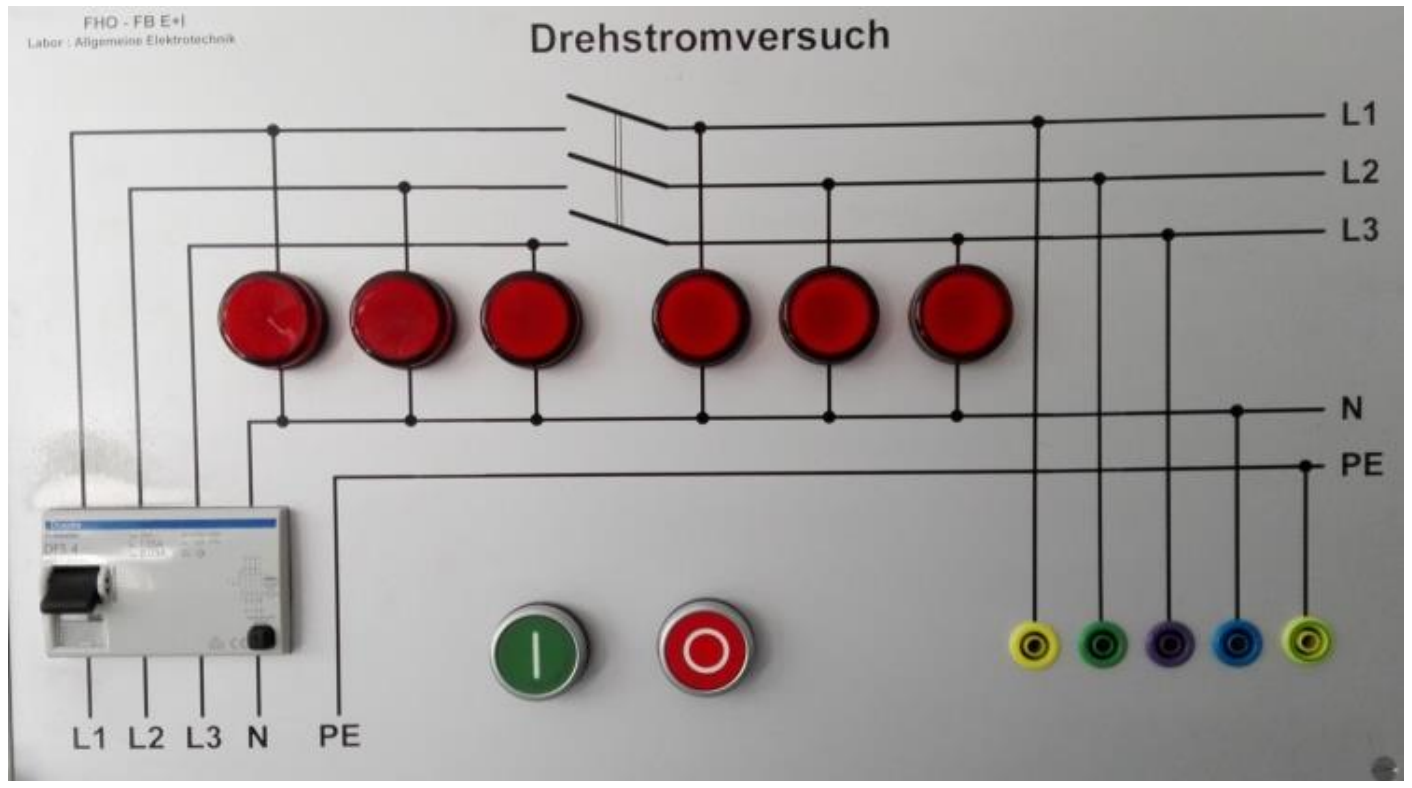
\includegraphics[width=0.5\textwidth]{img/img2.1.1.png}
      \end{center}
      \caption{Netzmodell am Versuchstisch }\label{img2.1.1}
    \end{figure}
    
    	\begin{figure}[h!]
    	\centering
    	\begin{subfigure}[b]{0.75\textwidth}
    		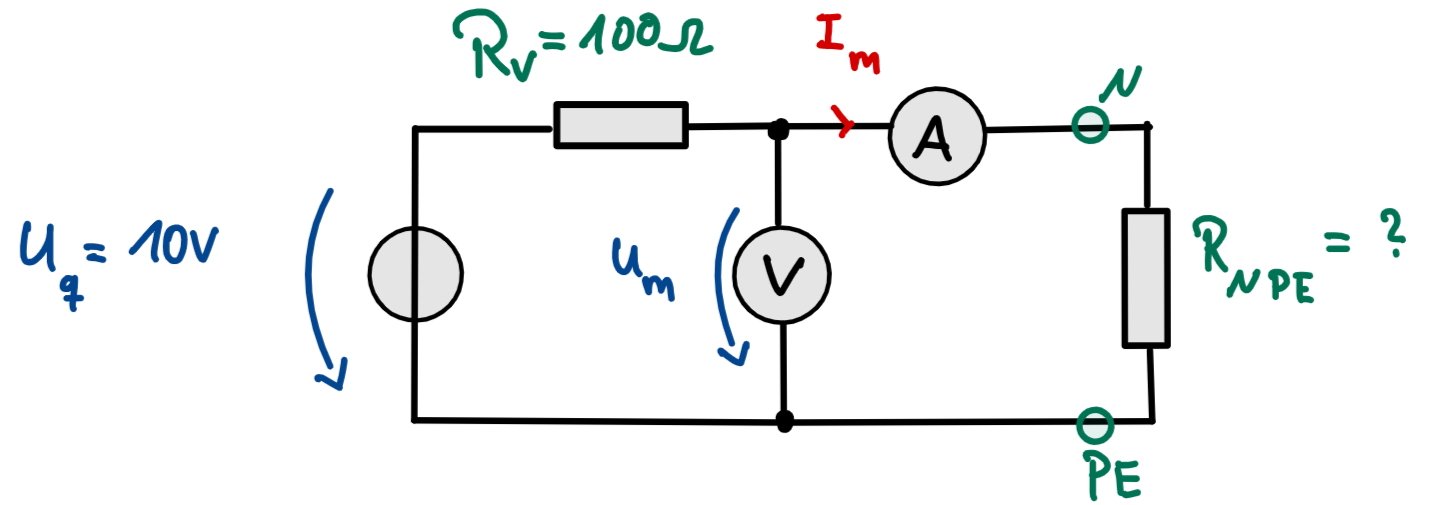
\includegraphics
    		[width=\textwidth]{img/img2.1.2.png}
    	\end{subfigure}
    	\caption{Skizze Messung, um Netzform zuermitteln}\label{img2.1.2}
    \end{figure}
    
  \item Skizzieren Sie eine Schaltung zur Bestimmung des Fehlerstromes des FI-Schutzschalters mit Hilfe des FI-Testers aus Abbildung \ref{img2.2.1} und Multimetern zur Strom- bzw. Spannungsmessung. 
	\begin{figure}[h!]
		\centering
		\begin{subfigure}[b]{0.5\textwidth}
			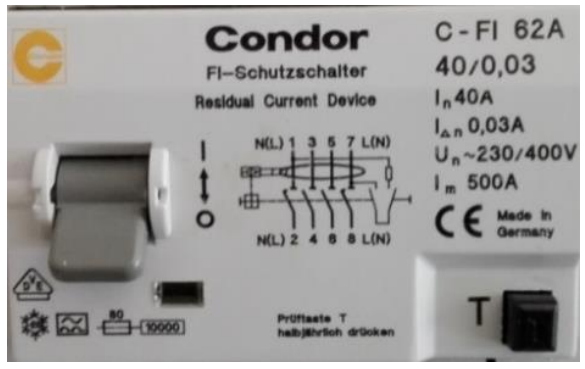
\includegraphics
			[width=\textwidth]{img/img2.2.1.png}
		\end{subfigure}\hfil
		\begin{subfigure}[b]{0.5\textwidth}
		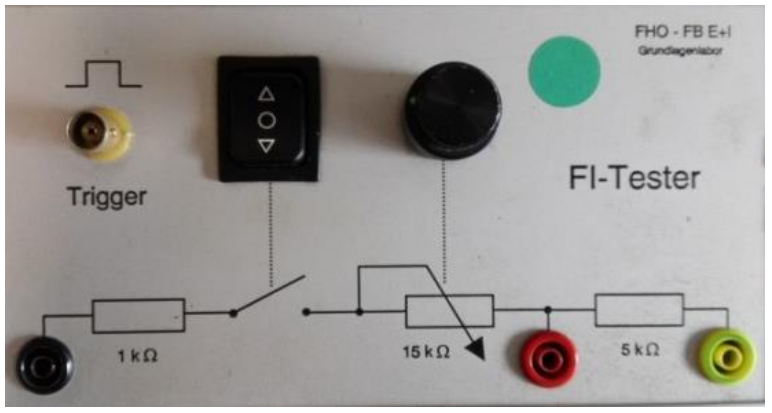
\includegraphics
		[width=\textwidth]{img/img2.2.2.png}
		\end{subfigure}
	\caption{FI-Schutzschalter und FI-Tester}\label{img2.2.1}
	\end{figure}
	
	Der FI-Tester wird an einen Außenleiter, den Neutralleiter und die Erde angeschlossen. Im Tester sind drei Widerstände in Reihe geschaltet, die über drei Anschlusspunkte verfügen. Der Lastwiderstand und der variable Widerstand werden zwischen dem Neutralleiter und L1 angeschlossen, während der Fehler-Widerstand parallel dazu geschaltet ist.\\

	\begin{figure}[h!]
		\begin{center}
			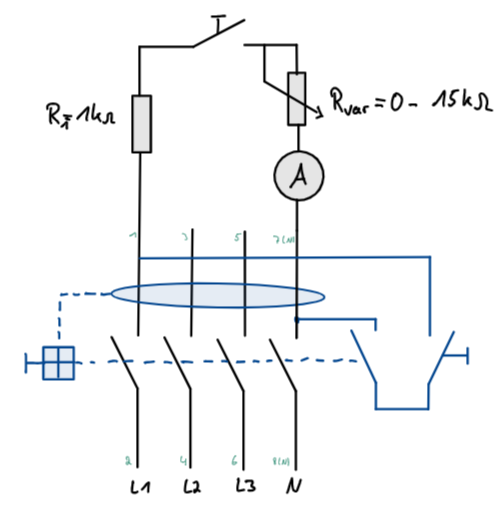
\includegraphics[width=0.75\textwidth]{img/img2.2.3.png}
		\end{center}
		\caption{Fehlerstrommessung am FI-Schutzschalter mit FI-Tester und Multimetern}\label{img2.2.3}
	\end{figure}
  \pagebreak
	

	% {
	% % \renewcommand{\abstractname}{Herleitung zum FI-Tester}
 %  \centering{Herleitung zum FI-Tester}\\\ \\
	% % % \begin{abstract}
	% 	\fcolorbox{black}{lightgray}{\parbox{\linewidth}{
	% 			\begin{align*}			
 %          I_{fehler}&=I_{ges}\cdot \frac{R_v+R_{var}}{R_{fehler}}\\ 
 %          I_{ges} &=\frac{U}{R_{ges}}\\ 
 %          I_{ges} &=\frac{U}{\frac{R_{fehler}\cdot(R_v+R_{var)}}{R_{fehler}+(R_v+R_{var})}}\\
 %          I_{ges} &={U}\cdot{\frac{R_{fehler}+R_v+R_{var}}{R_{fehler}\cdot(R_v+R_{var})}}\\
 %          I_{fehler}&={U}\cdot{\frac{R_{fehler}+R_v+R_{var}}{R_{fehler}\cdot(R_v+R_{var})}}\cdot \frac{R_v+R_{var}}{R_{fehler}}\\ 
 %          I_{fehler}&={U}\cdot{\frac{R_{fehler}+R_v+R_{var}}{(R_{fehler})^2}}\\
 %          I_{fehler}&={230\ V}\cdot{\frac{5\ k\Omega+1\ k\Omega+R_{var}}{(5\ k\Omega)^2}}\\
 %          I_{fehler}&={230\ V}\cdot{\frac{6\ k\Omega+R_{var}}{25\ (k\Omega)^2}}\\
 %          R_{var}&=\frac{I_{fehler}\cdot{25\ (k\Omega)^2}}{230\ V}-6\ k\Omega\\
 %          R_{var}&=\frac{15\ mA\cdot{25\ (k\Omega)^2}}{230\ V}-6\ k\Omega\\
	% 			\end{align*}
	% 		}}
	% % \end{abstract}
	% }
	
	Das Hauptziel besteht darin, den FI-Schutzschalter auszulösen, sobald ein Differenzstrom von mehr als 30 mA auftritt. Aus diesem Grund muss der Wert des variablen Widerstands, der anfänglich bei 15k Ohm liegt, schrittweise verringert werden, bis der FI-Schalter auslöst.

  \item An einem Vierleiter-Drehstromnetz ist eine symmetrische ohmsch-induktive Last (Reihenschaltung von Induktivität und Widerstand) in Sternschaltung angeschlossen. Bestimmen Sie formelmäßig die nötige Kapazität in Parallelschaltung (Sternschaltung), um eine vollständige Kompensation ($\cos \varphi = 1$) zu erreichen. \\
\begin{align*}
  \underline Y &=\frac{1}{(R+j\omega L)}+ {j\omega C}\\
  \underline Y &=\frac{1+ j\omega C(R+j\omega L)}{R+j\omega L}\\
  \underline Y &=\frac{1-\omega^2 LC+ j\omega CR}{R+j\omega L}\\
  \underline Y &=\frac{(1-\omega^2 LC+ j\omega CR) \cdot(R+j\omega L)}{R^2+(\omega L)^2}\\
  \underline Y &=\frac{R-\omega^2 RLC - \omega^3 RLC}{R^2+(\omega L)^2} 
  + j \frac{\omega L - \omega^3CL^2+\omega CR^2}{R^2+(\omega L)^2}\\
  \underline Y_{komp} &=Re\{\underline Y\}=\frac{R-\omega^2 RLC - \omega^3 RLC}{R^2+(\omega L)^2} \\
  \Rightarrow Im\{\underline Y\}&=0\\
  \omega L - \omega^3CL^2+\omega CR^2 &= 0\\
  C\cdot(\omega^3L^2+\omega R^2) - \omega L  &= 0\\
  C &=\frac{\omega L}{\omega^3 L^2+\omega R^2}\\
  C_{Y} &=\frac{L}{\omega^2 L^2+R^2}
\end{align*}

  \item Bestimmen Sie formelmäßig die nötige Kapazität, wenn die Kondensatoren in Dreieck verschaltet sind.
    \begin{align*}
      C_{Y} &=\frac{L}{\omega^2 L^2+R^2}\\
      C_{\Delta} &= \frac{1}{3}\cdot C_{Y}\\
      C_{\Delta} &= \frac{1}{3}\cdot \frac{L}{\omega^2 L^2+R^2}\\
    \end{align*}

  \item\label{aufgabe2.5} An einem Vierleiter-Drehstromnetz mit der konstanten Außenleiterspannung $U = 380\ V$ sind nach Abbildung \ref{img2.6.1} unsymmetrische Lasten angeschlossen. Bestimmen Sie rechnerisch und graphisch den Strom im Nullleiter, legen Sie dazu $\underline{U_1}$ in die reelle Achse, $f = 50\ Hz$!
	\\ \ \\
	In einer Sternschaltung müssen wir die Außenleiterspannung in die Strangspannung umrechnen, da die Spannung über die Widerstände aufgeteilt wird und zudem eine Phasenverschiebung von 120 Grad zwischen den jeweiligen Spannungen besteht.\\
	\begin{align*}
		U_{Str} &= \frac{U}{\sqrt{3}} \\
		U_{Str} &= \frac{380\ V}{\sqrt{3}}\\
		U_{Str} &= 219,39\ V\\ \ \\
		U_{12}=220\ Ve^{j0^\circ} \hspace{1cm}
		U_{23}&=220\ Ve^{j120^\circ} \hspace{1cm}
		U_{31}=220\ Ve^{-j120^\circ}\\
	\end{align*}
		
	Die einzelnen komplexen Widerstände werden berechnet, um die Strangstromstärken zu ermitteln.
	
	\begin{align*}
		\underline{z}_{1} &= R_{1} + j\omega L_{1} = 1,47\ k\Omega + j2\pi\cdot 50\ Hz\cdot1,5\ H = 1,54\ k\Omega e^{j17,77^\circ}\\
		\underline{z}_{2} &= R_{2} = 2\ k\Omega = 2\ k\Omega e^{j0^\circ}\\
		\underline{z}_{3} &= R_{3} + \frac{1}{j\omega C_{3}} = 2,18\ k\Omega + \frac{1}{j2\pi\cdot 50\ Hz\cdot2\ \mu F} = 2,67\ k\Omega e^{-j36,13^\circ}\\
	\end{align*}
	
	Die zuvor ermittelten Werte werden jetzt genutzt, um die Strangströme zu berechnen.
	
	\begin{align*}
		\underline{I}_{1} &= \frac{\underline{U}_{12}}{\underline{z}_{1}} = 
    \frac{219,4\ Ve^{j0^\circ}}{1,54\ k\Omega e^{j17,77^\circ}}=0,14\ Ae^{-j17,77^\circ}\\ 
    \underline{I}_{1} &= \frac{\underline{U}_{23}}{\underline{z}_{2}} = 
    \frac{219,4\ Ve^{j120^\circ}}{4\ k\Omega e^{j0^\circ}}=0,109\ Ae^{j120^\circ}\\ 
    \underline{I}_{1} &= \frac{\underline{U}_{31}}{\underline{z}_{3}} = 
    \frac{219,4\ Ve^{-j120^\circ}}{2,67\ k\Omega e^{-j36,13^\circ}}=0,081\ Ae^{-j87,8^\circ}\\
		\sum I &= \underline{I_1}+\underline{I_2}+\underline{I_3}+\underline{I_N}=0\\
		\Rightarrow \underline{I_N}&=-(\underline{I_1}+\underline{I_2}+\underline{I_3})\\
    \underline{I_N} &= -(0,14\ Ae^{-j17,77^\circ}+0,109\ Ae^{j120^\circ}+0,081\ Ae^{-j87,8^\circ})\\ 
    \underline{I_N} &= -(0,087\ Ae^{-19,66^\circ})=0,087\ Ae^{160,34^\circ}

	\end{align*}
  \begin{figure}[h!]
    \begin{center}
      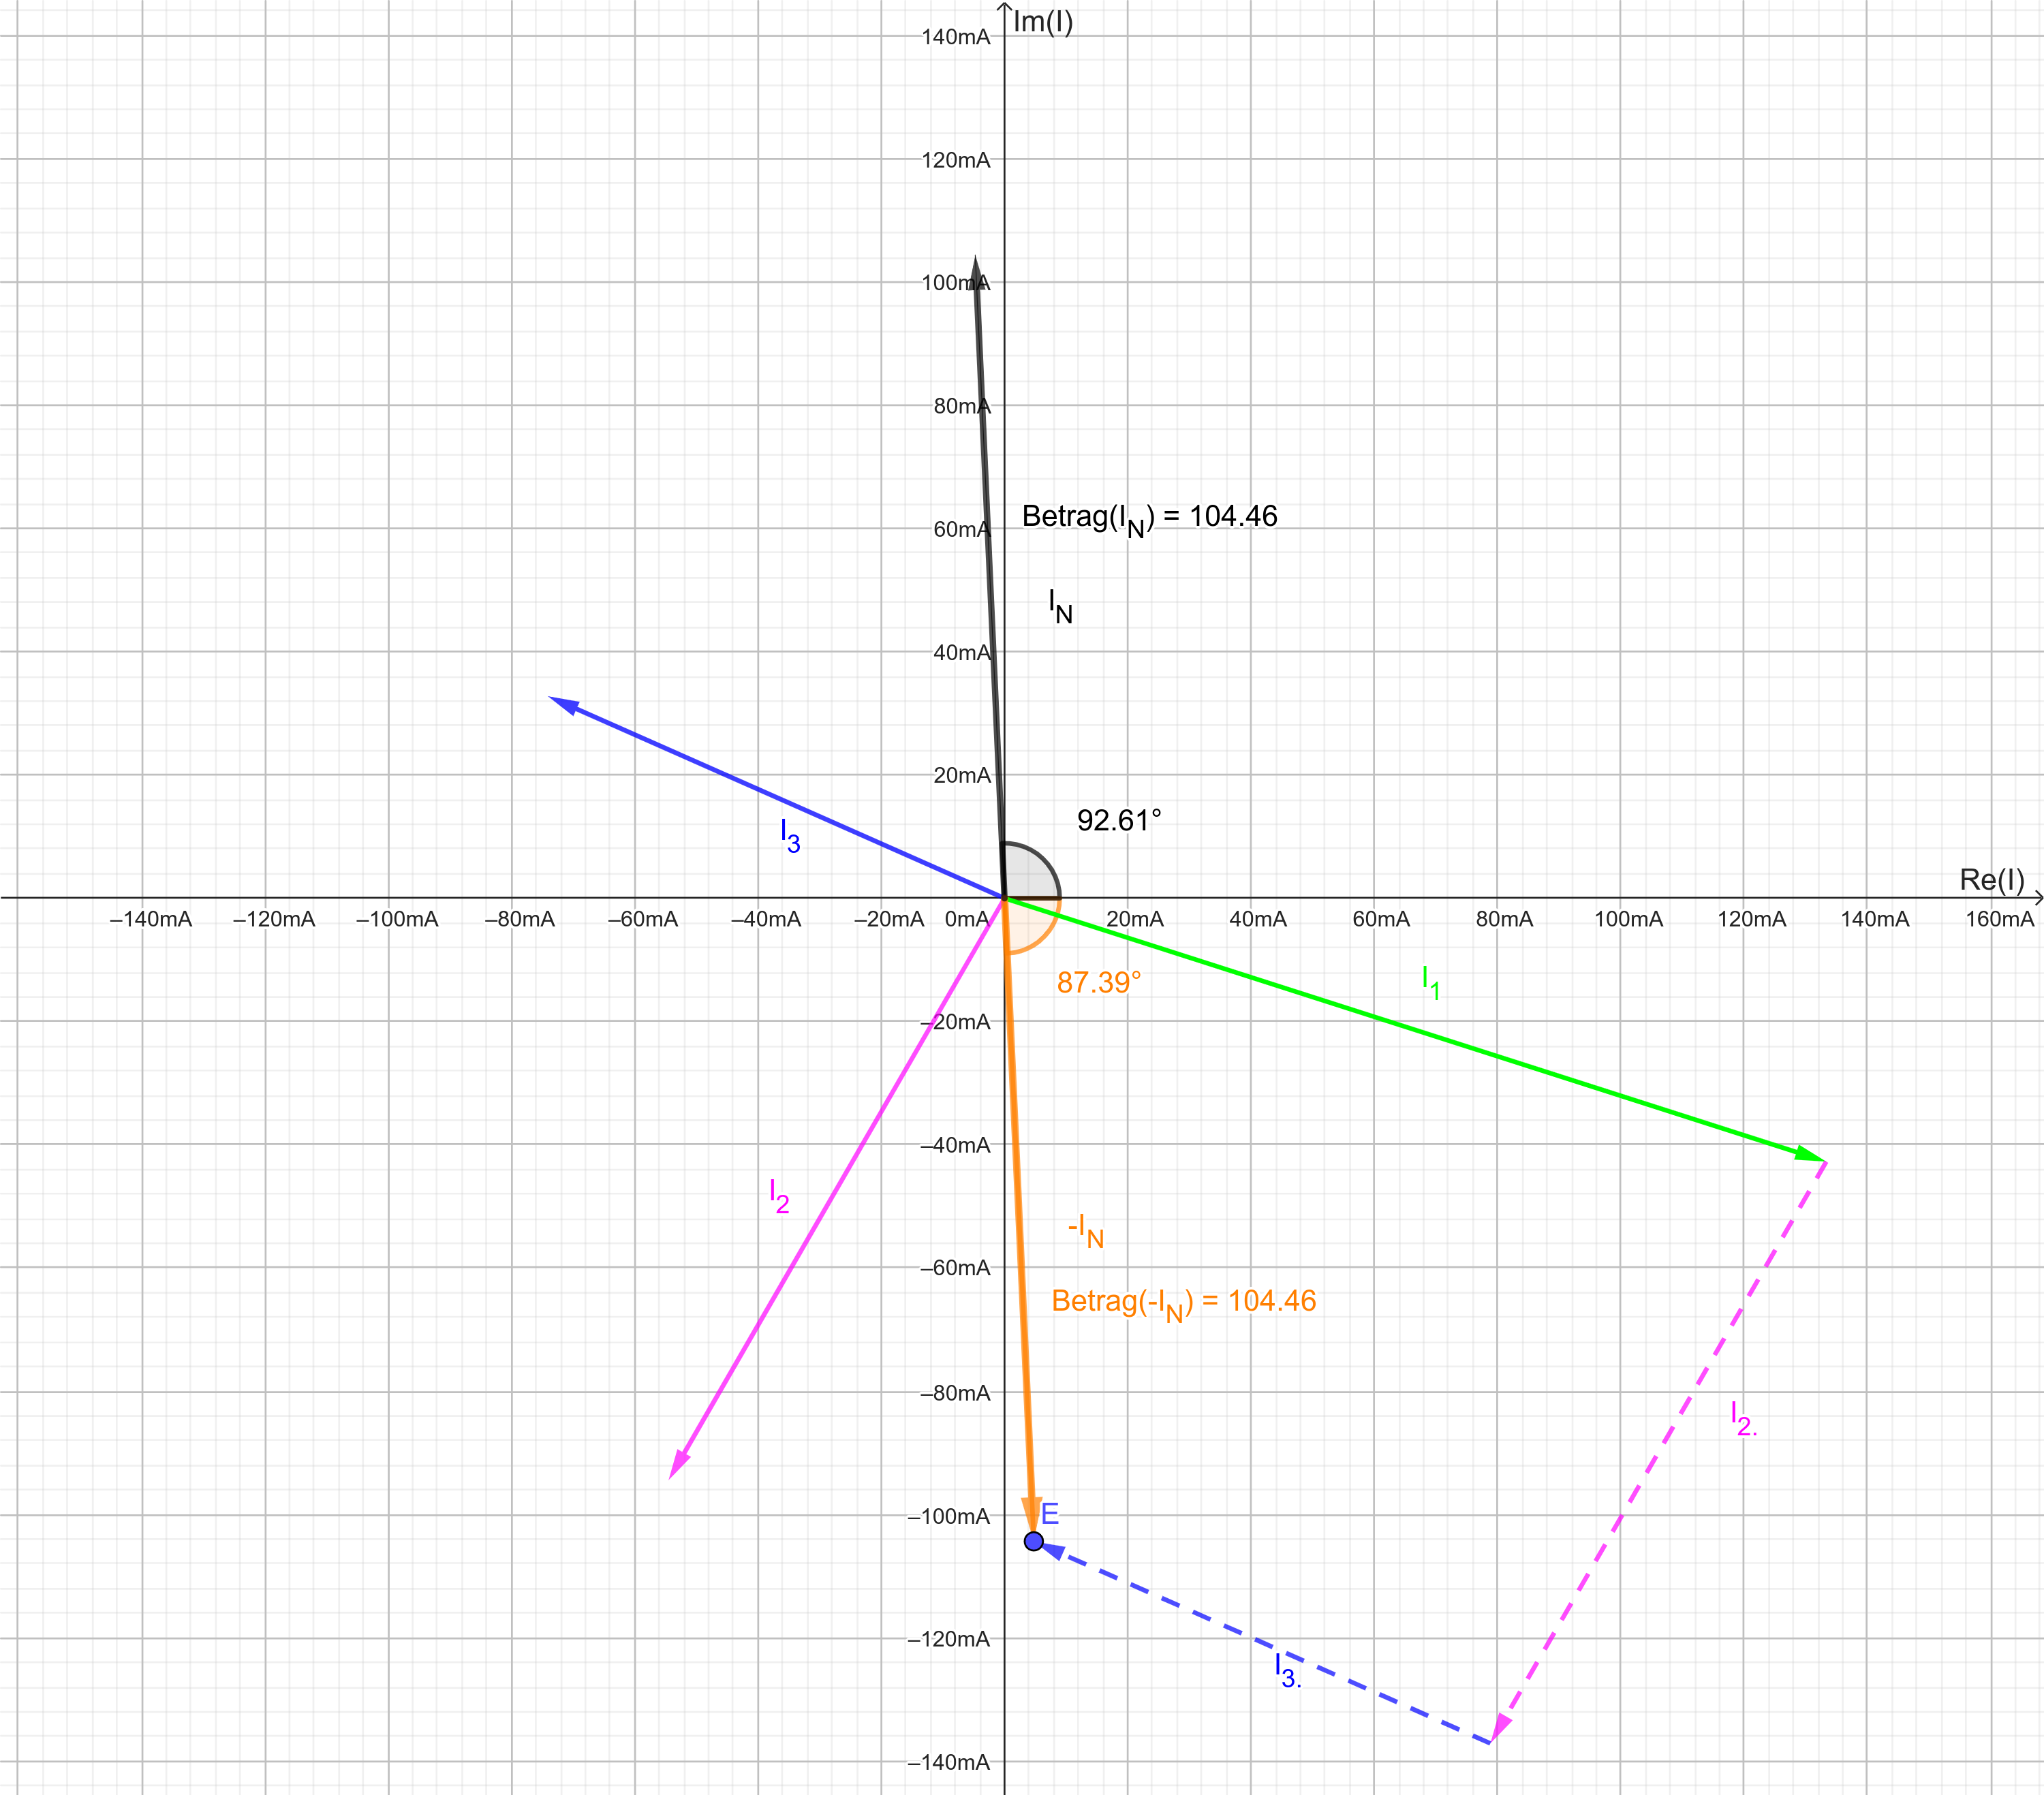
\includegraphics[width=0.70\textwidth]{img/img2.6.3.jpg}
    \end{center}
    \caption{Aufgabe \ref{aufgabe2.5} $I_1,\ I_2,\ I_3\text{ und }I_N$}
  \end{figure}
\pagebreak	
\item Bestimmen Sie nun für dieselbe Last alle Ströme und Spannungen ohne angeschlossenen Neutralleiter. Zeichnen Sie das Zeigerdiagramm der Spannungen $\underline{U_{1K}},\ \underline{U_{2K}} \text{ und } \underline{U_{3K}}$. \\\ \\
  \textbf{Leitfähigkeit:}
  \begin{align*}
    \underline{Y_1} &=\frac{1}{R_1+j\omega L_1} =\frac{1}{1,47\ k\Omega+j2\pi\cdot 50\ Hz \cdot1,5\ H} =0,617\ mS -j 0,198\ mS\\
    \underline{Y_2} &=\frac{1}{R_2} = \frac{1}{2\ k\Omega} = 0,5\ mS\\
    \underline{Y_3} &=\frac{1}{R_3-j\frac{1}{ j\omega C_3}}=\frac{1}{2,18\ k\Omega-j\frac{1}{2\pi\cdot 50\ Hz\cdot2\ \mu F}}
    = 0,299\ mS + j 0,218\ mS\\
    \underline{Y} &={\underline{Y_1}+\underline{Y_2}+\underline{Y_3}}=1,416\ mS+ j0,02\ mS= 1,416\ mS\cdot e^{j0,81^\circ}
  \end{align*}
  \textbf{Sternpunktspannung:}
    $$\underline{U_{KN}}=\frac{\underline{Y_1}\cdot\underline{U_{1N}}+\underline{Y_2}\cdot\underline{U_{2N}}+\underline{Y_3}\cdot\underline{U_{3N}}}{\underline{Y}}$$
      \begin{multline*}
    \underline{U_{KN}}=\left(0,648\ mS\cdot e^{-j17,79^\circ}\cdot 219,39\ V e^{j0} \right .
                      +0,5\ mS\cdot e^{j0}\cdot 219,39\ V e^{j120^\circ}\\
                      \left . +0,37\ mS\cdot e^{j36,1^\circ}\cdot 219,39\ V e^{-j120^\circ}\right)
                      \cdot\frac{1}{1,416\ mS\cdot e^{j0,81^\circ}}
    \end{multline*}
    $$\underline{U_{KN}}=62,66\ V-j21,48\ V=66,236\ V e^{-j18,92^\circ}$$
  \textbf{Spannungsmaschen:}
  \begin{align*}
    \underline{U_{1K}} &= \underline{U_{1N}} - \underline{U_{KN}} = 219,39\ Ve^{j0^\circ} - 66,236\ Ve^{-j18,92^\circ}\\
    \underline{U_{1K}} &= 158,2\ Ve^{j7,8^\circ}\\
    \underline{U_{2K}} &= \underline{U_{2N}} - \underline{U_{KN}} = 219,39\ Ve^{j120^\circ} - 66,236\ Ve^{-j18,92^\circ}\\
    \underline{U_{2K}} &= 272,81\ Ve^{j129,18^\circ}\\
    \underline{U_{3K}} &= \underline{U_{3N}} - \underline{U_{KN}} = 219,39\ Ve^{-j120^\circ} - 66,236\ Ve^{-j18,92^\circ}\\
    \underline{U_{3K}} &= 241,05\ Ve^{-j135,74^\circ}
  \end{align*}
  \textbf{Ströme:}
  \begin{align*}
    \underline{I_1} &= \underline{Y_1}\cdot\underline{U_{1K}} = 0,648\ mS\cdot e^{-j17,79^\circ}\cdot 158,2\ Ve^{j7,8^\circ}\\
    \underline{I_1} &= 102,5\ mA \cdot e^{-j9,99^\circ}\\
    \underline{I_2} &= \underline{Y_1}\cdot\underline{U_{1K}} = 0,5\ mS\cdot e^{j0}\cdot 272,81\ Ve^{j129,18^\circ}\\
    \underline{I_2} &= 136,41\ mA\cdot e^{j129,18^\circ}\\
    \underline{I_3} &= \underline{Y_1}\cdot\underline{U_{1K}} = 0,37\ mS\cdot e^{j36,1^\circ}\cdot 241,05\ Ve^{j-135,74^\circ}\\
    \underline{I_3} &= 89,19\ mA\cdot e^{-j99,55^\circ}\\
    \underline{I_1} +\underline{I_2} + \underline{I_3} &\approx 0
  \end{align*}
\begin{figure}[h!]
  \begin{center}
    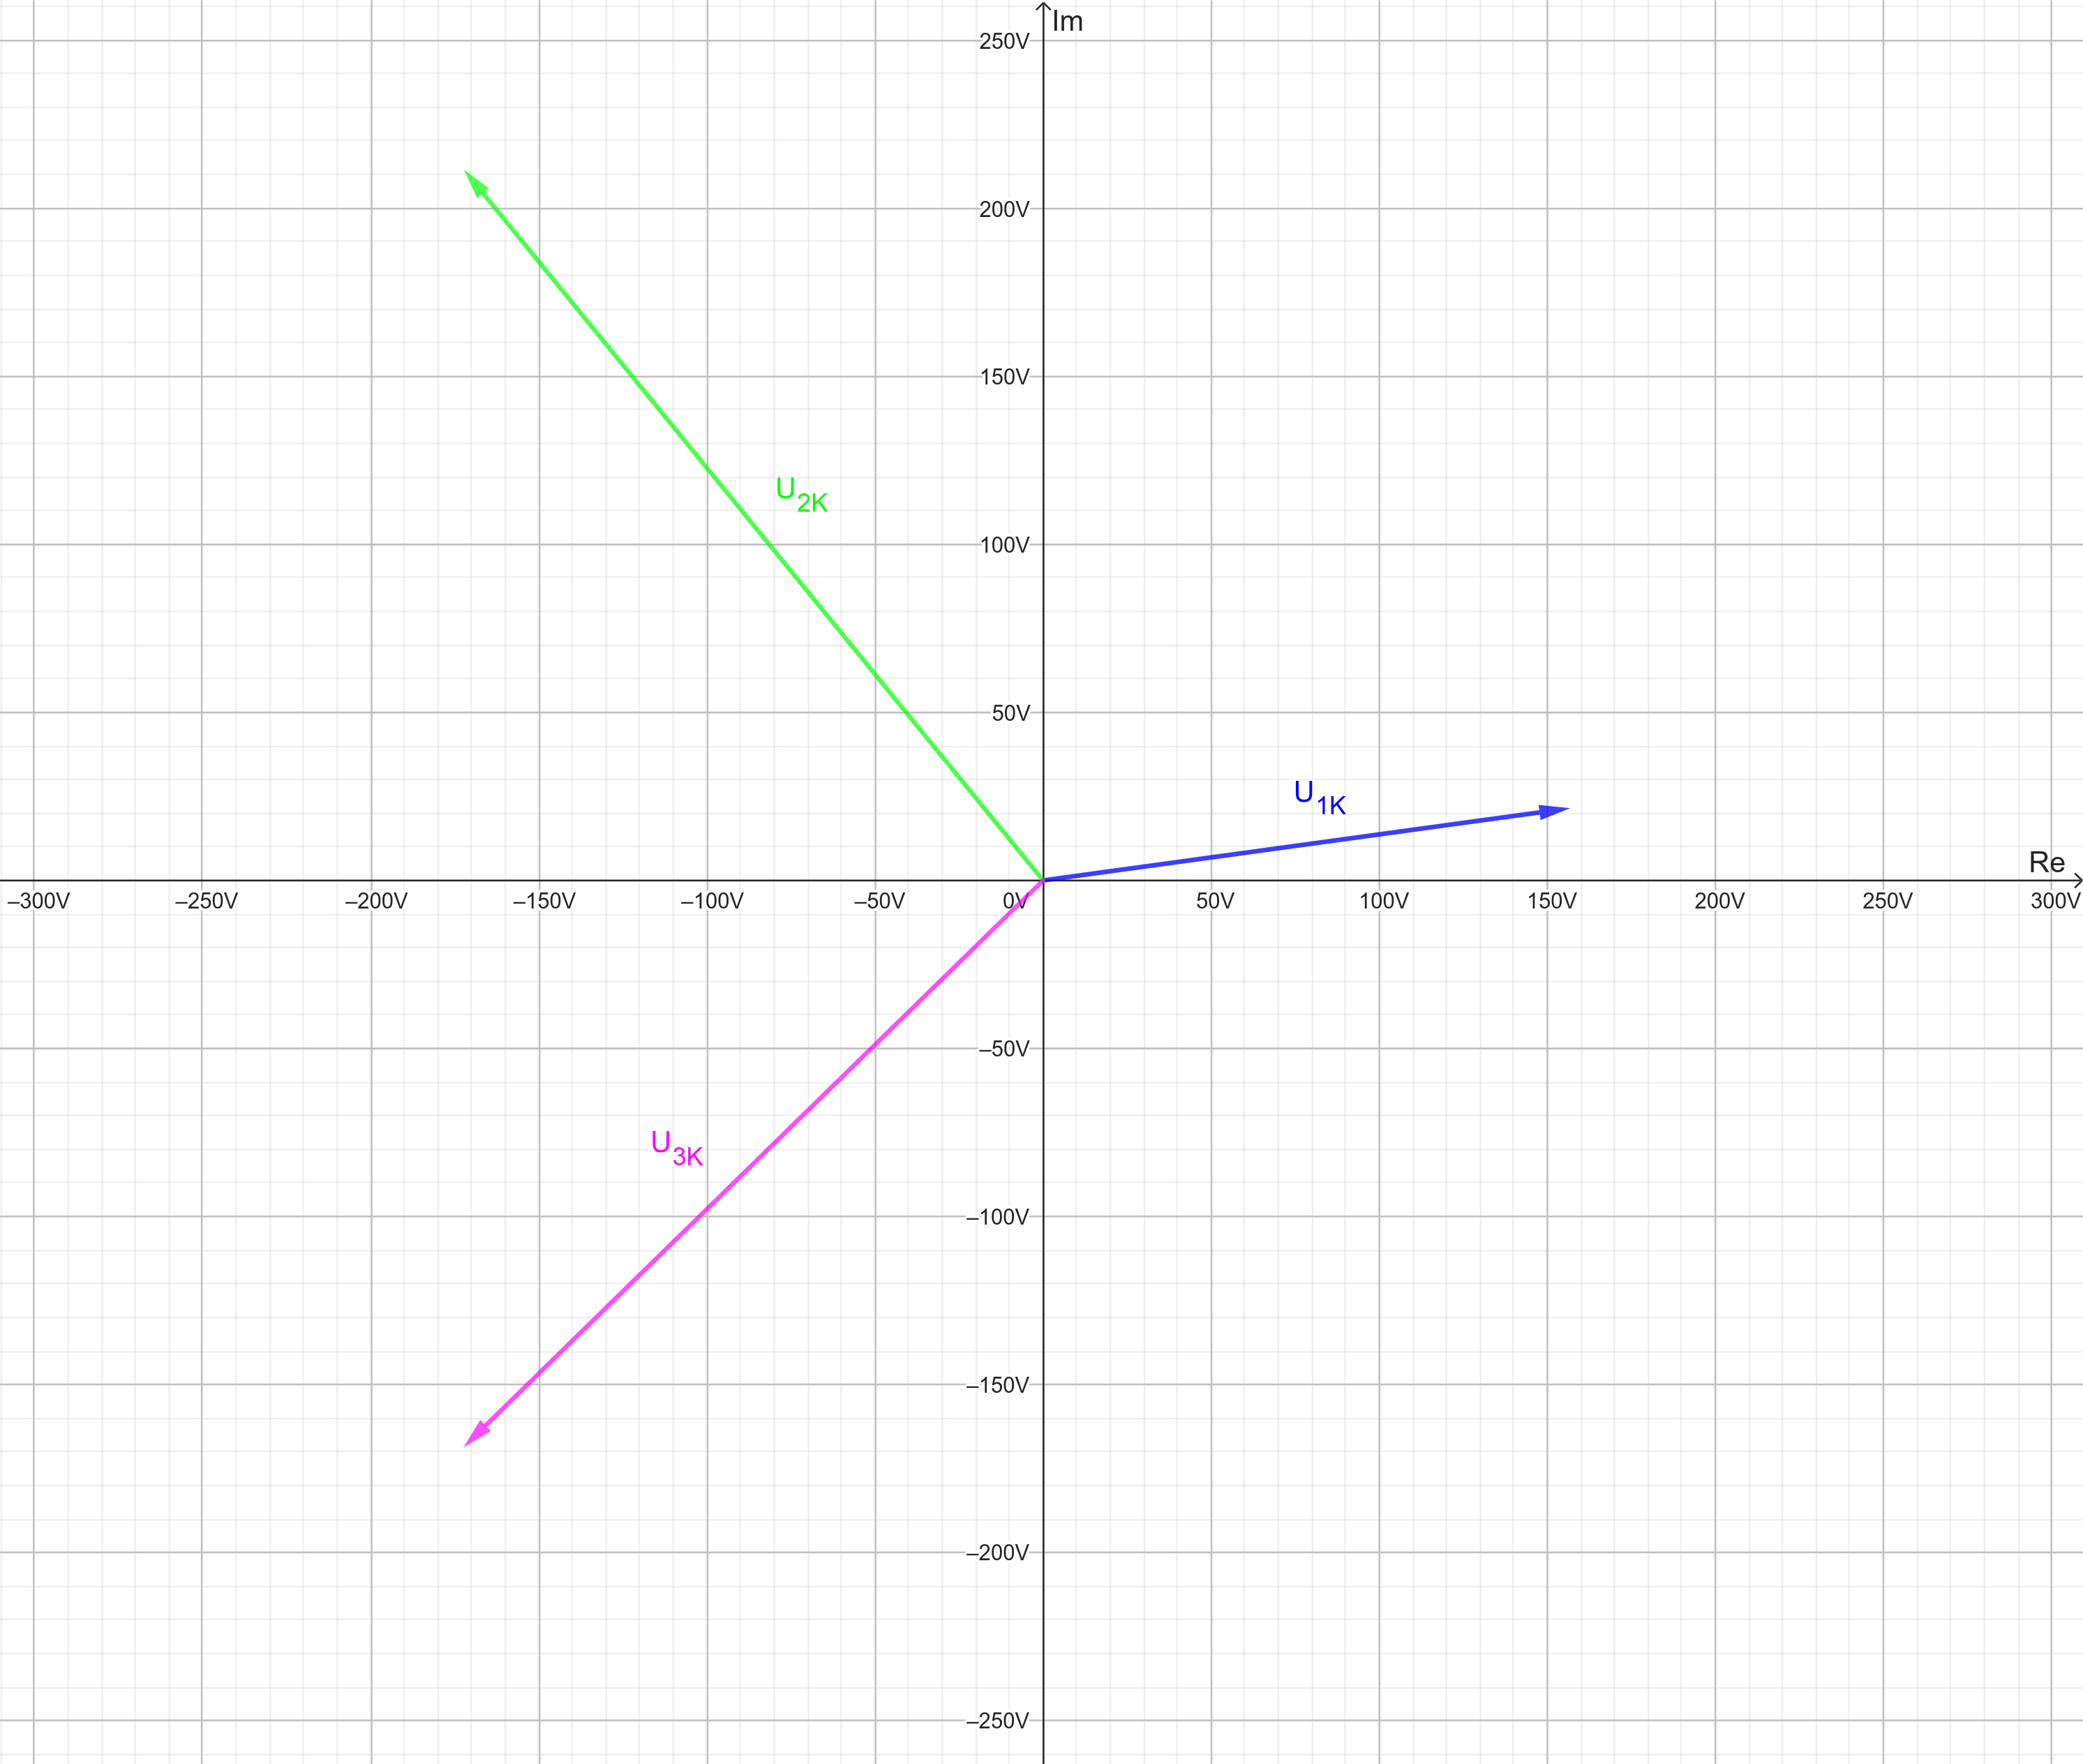
\includegraphics[width=0.70\textwidth]{img/img2.6.2.png}
  \end{center}
  \caption{Zeigerdiagramm der Spannungen $\underline{U_{1K}},\ \underline{U_{2K}} \text{ und } \underline{U_{3K}}$}
\end{figure}

\pagebreak	
\ 
  \begin{figure}[h!]
    \begin{center}
      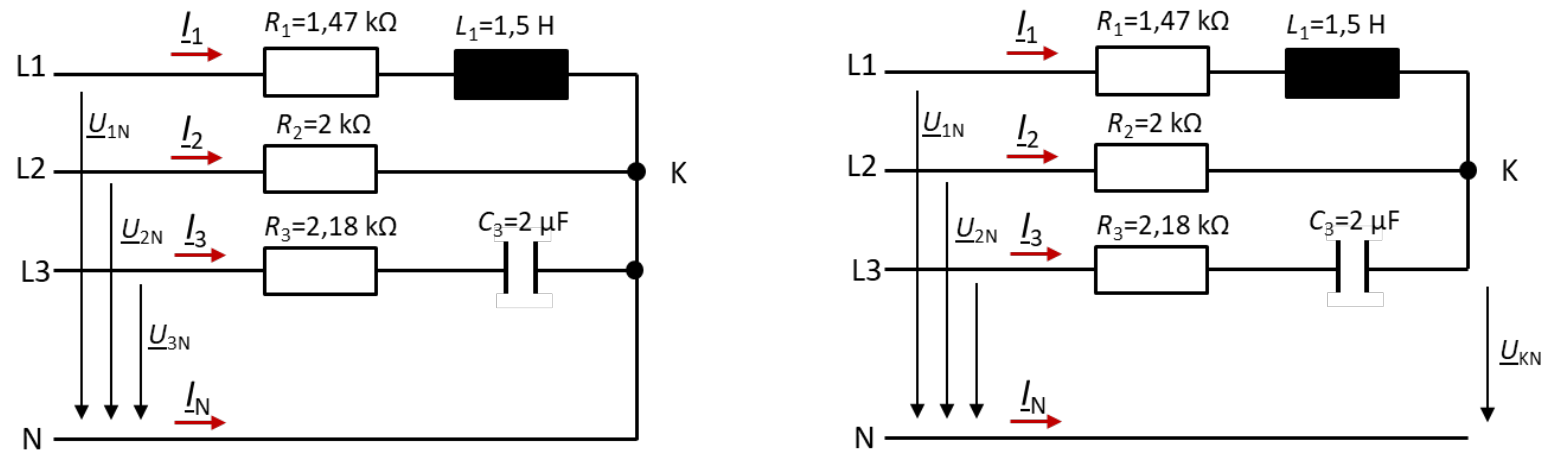
\includegraphics[width=0.95\textwidth]{img/img2.6.1.png}
    \end{center}
    \caption{Last a mit und ohne angeschlossenen Neutralleiter (Gruppe XXa)}\label{img2.6.1}
  \end{figure}
  
\end{enumerate}
